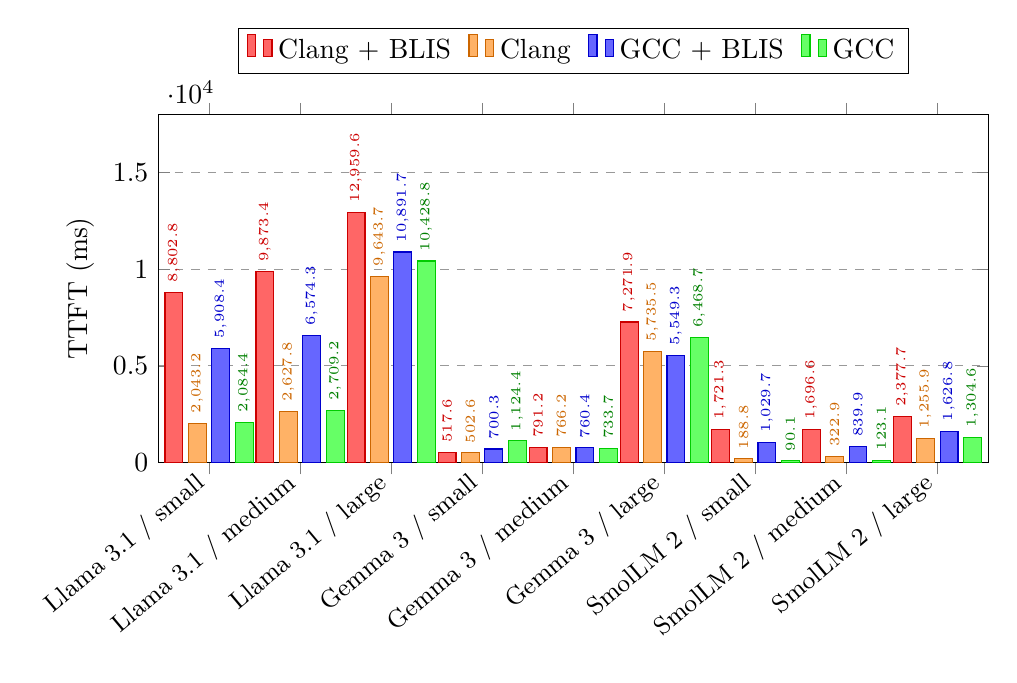
\begin{tikzpicture}
    \begin{axis}[
        % Plot type
        ybar,
        % Plot dimensions
        width            = \textwidth,
        height           = 6cm,
        enlarge x limits = 0.07,
        bar width        = 1.5ex,
        % Labels
        ylabel            = {TTFT (ms)},
        symbolic x coords = {
            {Llama 3.1 / small},
            {Llama 3.1 / medium},
            {Llama 3.1 / large},
            {Gemma 3 / small},
            {Gemma 3 / medium},
            {Gemma 3 / large},
            {SmolLM 2 / small},
            {SmolLM 2 / medium},
            {SmolLM 2 / large}
        },
        x tick label style = {rotate = 40, anchor = east, font = \small},
        % Axes
        ymin = 0,
        ymax = 18000,
        % Labels
        nodes near coords,
        nodes near coords style={
            font   = \tiny,
            rotate = 90,
            anchor = west,
            /pgf/number format/fixed,
            /pgf/number format/precision = 1
        },
        % Grid
        ymajorgrids = true,
        grid style  = {dashed, gray!80},
        % Legend
        legend style = {
            at={(0.5, 1.25)},
            anchor         = north,
            legend columns = 4,
            /tikz/every even column/.append style={column sep = 1ex}
        }
    ]

        % Clang BLIS
        \addplot+[
            % Bar and label color
            fill                                = red!60,
            draw                                = red!80!black,
            every node near coord/.append style = {color = red!80!black}
        ] coordinates {
            ({Llama 3.1 / small},  8802.80)
            ({Llama 3.1 / medium}, 9873.40)
            ({Llama 3.1 / large}, 12959.57)
            ({Gemma 3 / small},     517.56)
            ({Gemma 3 / medium},    791.24)
            ({Gemma 3 / large},    7271.87)
            ({SmolLM 2 / small},   1721.33)
            ({SmolLM 2 / medium},  1696.59)
            ({SmolLM 2 / large},   2377.65)
        };

        % Clang CPU
        \addplot+[
            % Bar and label color
            fill                                = orange!60,
            draw                                = orange!80!black,
            every node near coord/.append style = {color = orange!80!black}
        ] coordinates {
            ({Llama 3.1 / small},  2043.19)
            ({Llama 3.1 / medium}, 2627.81)
            ({Llama 3.1 / large},  9643.68)
            ({Gemma 3 / small},     502.59)
            ({Gemma 3 / medium},    766.18)
            ({Gemma 3 / large},    5735.50)
            ({SmolLM 2 / small},    188.78)
            ({SmolLM 2 / medium},   322.90)
            ({SmolLM 2 / large},   1255.93)
        };

        % GCC BLIS
        \addplot+[
            % Bar and label color
            fill                                = blue!60,
            draw                                = blue!80!black,
            every node near coord/.append style = {color = blue!80!black}
        ] coordinates {
            ({Llama 3.1 / small},  5908.42)
            ({Llama 3.1 / medium}, 6574.28)
            ({Llama 3.1 / large}, 10891.71)
            ({Gemma 3 / small},     700.34)
            ({Gemma 3 / medium},    760.35)
            ({Gemma 3 / large},    5549.34)
            ({SmolLM 2 / small},   1029.68)
            ({SmolLM 2 / medium},   839.86)
            ({SmolLM 2 / large},   1626.84)
        };

        % GCC CPU
        \addplot+[
            % Bar and label color
            fill                                = green!60,
            draw                                = green!80!black,
            every node near coord/.append style = {color = green!50!black}
        ] coordinates {
            ({Llama 3.1 / small},  2084.42)
            ({Llama 3.1 / medium}, 2709.15)
            ({Llama 3.1 / large}, 10428.83)
            ({Gemma 3 / small},    1124.44)
            ({Gemma 3 / medium},    733.71)
            ({Gemma 3 / large},    6468.68)
            ({SmolLM 2 / small},     90.06)
            ({SmolLM 2 / medium},   123.14)
            ({SmolLM 2 / large},   1304.62)
        };

        \legend{Clang + BLIS, Clang, GCC + BLIS, GCC}
    \end{axis}
\end{tikzpicture}
